\chapter{Theorie}
\begin{figure}[H]
\centering
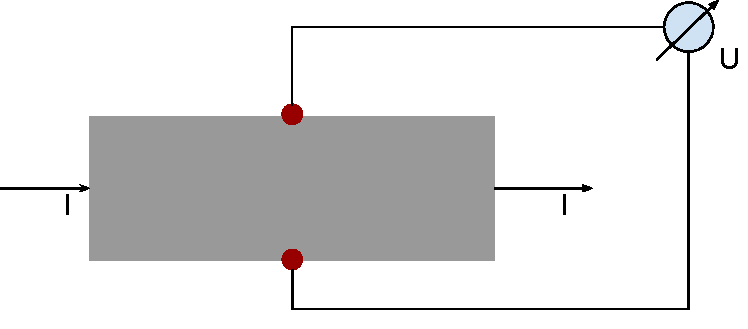
\includegraphics[width=0.6\textwidth]{img/halleffekt_plaettchen.pdf}
\caption{Halleffekt-Plättchen}
\end{figure}

\section{Driftgeschwindigkeit}
Schließt an einen elektrischen Leiter eine Ladungspumpe an, so entsteht entlang des Leiters ein elektrisches Feld. Durch das elektrische Feld erfahren die freien Elektronen im Leiter die Kraft:
$$F_{el} = E \cdot e$$

Die durch diese Kraft beschleunigten Teilchen stoßen mit übrigen Teilen des Leiters zusammen. Es stellt sich eine Durchschnittsgeschwindigkeit im Leiter ein.
Diese Geschwindigkeit nennt man \emph{Driftgeschwindigkeit} der Elektronen.

Wir betrachten ein Leiterplättchen mit der Breite $s$ und der Höhe $h$.
Fließt Strom durch das Plättchen, bewegen sich alle Elektronen im Leiter mit $\vec{v}$ Richtung Pluspol. Dafür benötigen sie die Zeit
$$t = \frac{s}{v}$$
In dieser Zeit übertragen alle $N$ strömenden Elektronen die Ladung 
$$Q = N \cdot e$$ 
Dabei fließt die Stromstärke
$$I = \frac{Q}{t} = \frac{N \cdot e}{s} \cdot v$$
Dabei ist $\frac{N \cdot e}{s}$ konstant. Daraus folgt
$$I \sim v$$

\section{Halleffekt}
Wird das stromdurchflossene Leiterplättchen senkrecht zur Bewegungsrichtung der Elektronen mit einem Magnetfeld durchsetzt, erfahren die Elektronen jeweils die Lorentzkraft
$$F_L = B \cdot e \cdot v$$
Die Elektronen wandern also auf eine Seite des Leiters. Wenn die Elektronen z.~B. von links nach rechts strömen, das Magnetfeld von vorne nach hinten zeigt, wandern die Elektronen nach der Drei-Finger-Regel der linken Hand nach unten. Dieses Phänomen wird \emph{Halleffekt} genannt.

\begin{figure}[H]
\centering
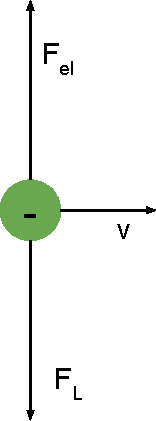
\includegraphics[width=0.15\textwidth]{img/halleffekt_kraft.pdf}
\caption{Kräftediagramm für ein Elektron im Hallplättchen}
\end{figure}

Die Elektronen „sammeln“ sich an einer Seite. Durch diese Ladungsverschiebung entsteht im Leiterplättchen ein elektrisches Feld. Nach kurzer Zeit stellt sich das Kräftegleichgewicht
$$F_L = F_{el}$$
ein. Die weiteren Elektronen durchlaufen das Plättchen also geradlinig.
Misst man an zwei direkt gegenüberliegenden Punkten oben und unten am Plättchen die Spannung, erhält man die Hallspannung $U_H$.

Nach der Formel für die Spannung eines Elektrischen Feldes $E = \frac{U}{d}$ ergibt sich für $U_H$:
$$U_H = E \cdot h$$
E lässt sich aus der Kraft, die das Feld auf die Elektronen ausübt bestimmen. Da diese Kraft im Gleichgewicht mit der Lorentzkraft steht, gilt für die Feldstärke $E$
$$E = \frac{F_L}{e}$$
$$E = B \cdot v$$

Für die Hallspannung gilt dann dementsprechend:
$$U_H = B \cdot v \cdot h$$

Mit dem oben beschriebenen Zusammenhang von $I$ und $v$ ergibt sich:
\begin{align*}
v &= \frac{I \cdot s}{N \cdot e} \\
U_H &= B \cdot h \cdot \frac{I \cdot s}{N \cdot e} \\
\end{align*}

Die Anzahl der Ladungsträger $N$ wird für das entsprechende Material des Leiterplättchens in Abhängigkeit vom Volumen als $n$ angegeben:
\begin{align*}
n &= \frac{N}{V} \\
n &= \frac{N}{h \cdot s \cdot d} \\
N &= n \cdot h \cdot s \cdot d \\
\end{align*}

Somit gilt für die Hallspannung:
$$U_H = B \cdot \frac{I}{n \cdot d \cdot e}$$